\section{Experiment} \label{sec:Experiment}

    \subsection{Velocity of ultrasound in polyacryl} \label{subsec:schallgeschwindigkeit}

        To measure the propagation speed of sound waves through media, three polyacryl cylinders with different lenghts were used. The time that the wave
        took to travel through the cylinder was measured via the method of reflection, where the ultrasound transmitter also worked as the detector of the signal.
        The time was then captured with the echoscope. With the method of reflection one has to notice that the length in the formula for the propagation speed
        is no double the length of the cylinder, concluding in:

        \begin{equation}
            v_{poly} = \frac{2 \cdot l}{\Delta t}
            \label{eq:schallgeschwindigkeit}
        \end{equation}
        \noindent
        As noted above l is the total length of the cylinder, $\Delta t$ is the time the wave took to travel twice through the cylinder and $v_{poly}$ is the
        resulting speed of sound. \\
        This method was then applied to all three different cylinder-lengths, each with three different frequencies $f_{1MHz} = 1 MHz$, $f_{2MHz} = 2 MHz$
        and $f_{4MHz} = 4 MHz$. Since the absorption for $f_{4MHz}$ was big, the largest cylinder could not be measured. \\
        With the relevant data shown in \ref{subsec:AppendixA}, Tab. \ref{tab:DataSchallgeschwindigkeit} the mean sound velocitys for each frequency is calculated:

        \begin{equation*}
        \begin{split}
            v_{poly. 1MHz} & = (2.619 \pm 0.032) \frac{km}{s}\\
            v_{poly. 2MHz} & = (2.677 \pm 0.033) \frac{km}{s}\\
            v_{poly. 4MHz} & = (2.746 \pm 0.052) \frac{km}{s}
        \end{split}
        \end{equation*}

        It is clearly visible, that the speed of sound in polyacryl depends on the frequency of the wave traveling through it. Thus it indicates dispersion in
        the sound velocity. \\
        In the data sheet from a manufacutrer, the longitunal wave velocity for the frequency of 1Mhz is given by
        $v_{poly,Lit} = 2.7 \frac{km}{s}$ \cite{SchallgeschwindigkeitPolyacryl}, therefore the measured value does not match the literature within the error.
        This could be due to the fact that the measurement was done in saturation of the used piezoelectric ultrasound emitter. Also because of the absorption 
        of the material, the gain on the echoscope had to be increased, which also increased the noise of the measurement thus increasing the uncertainty.
        
    \subsection{Absorption of ultrasound in PVC} \label{subsec:absorption}

        The coefficient of absorption is a material-specific quantity which indicates how strongly a wave is attenuated propagading a medium. The attenuation follows an exponetial behavior.
        The intesity $I$ as a function of the distance $x$ can approximately be described by:

        \begin{equation}
            I(x) \sim e^{-\lambda x}
        \end{equation}

        where $\lambda$ is the absorption coefficient. To determine this coefficient, the signal's reflected amplitude was measured at different lengths of PVC cylinders. By fitting an
        exponential curve to the data, the absorption coefficient can be determined for the different frequencies. \\
        For the $f=1MHz$ messuarment, $\lambda_{1 MHz}$ was determined to be $\lambda_{1 MHz} = (0.0346 \pm 0.0313) \frac{1}{cm}$ and for $f=2MHz$ it was 
        $\lambda_{2 MHz} = (0.0443 \pm 0.1297) \frac{1}{cm}$.
        The absorption coefficient increases with the frequency, which is a common behavior in materials. This can be explained by the fact that atoms oscillate faster at higher frequencies, 
        leading to stronger scattering of the waves. The orderes wave increasingly transforms into disordered oscillations, resulting in energy loss. \\

    \subsection{Measurements on a polyacrylic test block} \label{subsec:Laengenmessung}
        
        \begin{figure}[H]
            \centering
            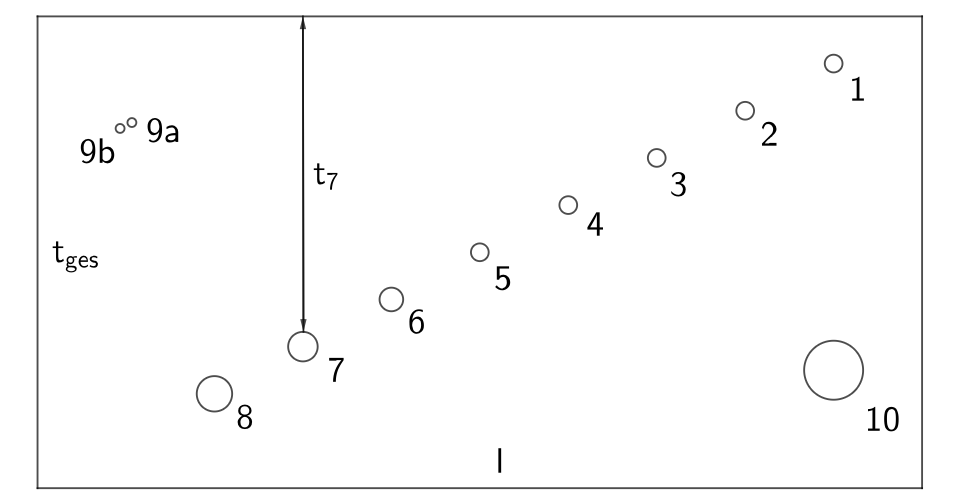
\includegraphics[width=0.5\textwidth]{../Images/Bildschirmfoto 2026-05-19 um 19.38.01.png}
            \caption{Schematics of the test block}
            \label{fig:testblock}
        \end{figure}

        As we know the speed of sound in polyacryl for the freuquency of $1MHz$ \ref{subsec:schallgeschwindigkeit}, we can use th echoscope to measure the depth $d_i$ of the holes in
         the test block. 
        We used the $1MHz$ Probe for a clear runtime measurement. The depth can be calculated from the time difference $\Delta t$ between the first and second reflection of the signal:

        \begin{equation}
            d_i = \frac{v_{poly,1MHz} \cdot \Delta t}{2}
        \end{equation}
        
        For reference, the depth were mearured with a caliper. The results are shown in tab. \ref{tab:Testwürfel}. 

        \begin{table}[H]
            \begin{tabular}{|c|c|c|c|}
            \hline
            $i$ & $d_{i,caliper}$ [mm] & $\Delta t$ [$\mu s$] & $d_{i}$ [mm] \\
            \hline
            1 & $(7.00 \pm 0.10)$ & $(5.825 \pm 0.010)$ & $(7.63 \pm 0.16)$ \\
            \hline
            2 & $(14.95 \pm 0.10)$ & $(11.606 \pm 0.010)$ & $(15.20 \pm 0.23)$ \\
            \hline
            3 & $(22.95 \pm 0.10)$ & $(17.574 \pm 0.010)$ & $(23.01 \pm 0.31)$ \\
            \hline
            4 & $(31.00 \pm 0.10)$ & $(23.358 \pm 0.010)$ & $(30.59 \pm 0.40)$ \\
            \hline
            5 & $(39.05 \pm 0.10)$ & $(29.489 \pm 0.010) $ & $(38.62 \pm 0.49)$ \\
            \hline
            6 & $(46.75 \pm 0.10)$ & $(35.182\pm 0.01)$ & $(46.07 \pm 0.58)$ \\
            \hline
            7 & $(54.15 \pm 0.10)$ & $(40.511 \pm 0.010)$ & $(53.05 \pm 0.66)$ \\
            \hline
            8 & $(61.65 \pm 0.10)$ & $(46.058 \pm 0.010)$ & $(60.31 \pm 0.75)$ \\
            \hline
            9a & $(17.45 \pm 0.10)$ & $(14.567 \pm 0.010)$ & $(19.08 \pm 0.27)$ \\
            \hline
            9b & $(19.10 \pm 0.10)$ & $(15.906 \pm 0.010)$ & $(20.83 \pm 0.29)$ \\
            \hline
            10 & $(55.45 \pm 0.10)$ & $(41.505 \pm 0.010)$ & $(54.35 \pm 0.68)$ \\
            \hline
            \end{tabular}
        \caption{Measurement of the testblock}
        \label{tab:Testwürfel}
        \end{table}

        Most measured values agree within their margin of error. However, it is noticeable that holes 9a and 9b show deviating values. This is due to the fact that the holes are located very 
        close to each other, meaning that a higher frequency would be beneficial in order to achieve a more precise resolution.

    \subsection{Resolution of an echoscope} \label{subsec:Aufloesungsvermoegen}

    As mentioned in \ref{subsec:Laengenmessung} can a higher frequency be used to achieve a better resolution. To determine the resolution of the echoscope, the distance between two holes, 
    $(9a$ und $9b)$, was measured with different frequencies. The resolution can be defined as the minimum distance between two holes, where they can still be distinguished as two separate holes. 
    Measurement for all three frequencies is shown in tab. \ref{tab:Resolution}.
    
    \begin{table}[H]
        \begin{tabular}{|c|c|}
        \hline
        Frequency & Distance $[mm]$\\
        \hline
        $2MHz$ & $(1.70 \pm 0.13)$ \\
        \hline
        $4MHz$ & $(1.75 \pm 0.14)$ \\
        \hline
        \end{tabular}
        \caption{Resolution of the echoscope}
        \label{tab:Resolution}
    \end{table}

    For a freuqueny of $1MHz$, the amplitude peaks could not be resolved as two distinct peaks; therefore, the distance between the reflectors could not be determined. In contrast, the measurements 
    performed at the higher frequencies showed a clear separation of the two peaks, making the distance measurable and allowing the axial resolution to be determined from the spacing 
    between the two holes.
    The resolution of the echoscope increases with increasing frequency, which is a characteristic behavior of ultrasound imaging systems. This can be explained by the shorter wavelengths associated 
    with higher frequencies, enabling improved spatial resolution and therefore a better distinction between closely spaced objects. However, higher frequencies are also subject to stronger 
    attenuation within the material, which reduces the penetration depth and consequently limits the effective measurement range in practical applications.
    
    
    \subsection{Spectral methods of an echoscope} \label{subsec:SpectraleMethoden}

    To investigate the spectral methods, the reflection signal of a polyacrylic plate was analyzed using the A-scan. In addition, an FFT and the cepstrum of the signal were evaluated in order to 
    determine the thickness of the plate.

    In the A-scan, several reflection peaks are visible, which originate from multiple reflections within the plate. After applying the FFT, approximately equidistant peaks appear in the frequency 
    spectrum. From the spacing $\Delta \nu$ between neighboring peaks, the pulse travel time can be determined using

    \[
    \Delta t = \frac{1}{\Delta \nu}.
    \]

    With the known speed of sound in the material, the thickness of the plate can then be calculated.

    In the cepstrum, only a few dominant peaks are visible, corresponding to the periodic travel-time components of the signal. This also allows the reflection distances to be determined.

    The results obtained from the FFT and the cepstrum agree within the error margins with the direct travel-time measurement and the measurement performed using a caliper.

    \subsection{Debye-Sears effect} \label{subsec:Dabye-Sears-Effekt}

        The Dabye-Sears effect describes an acousto-optic effect, where the ultrasound probe creates a standing wave with lattice constant $g = \lambda_S$
        perpendicular to an incoming laser beam. The beam then diffracts as it does with a classical optical lattice. With the formula for the
        lattice spectrum from classical optics one can determine the wavelength $\lambda_S$ of the ultrasound. \\

        \begin{figure}
            \centering
            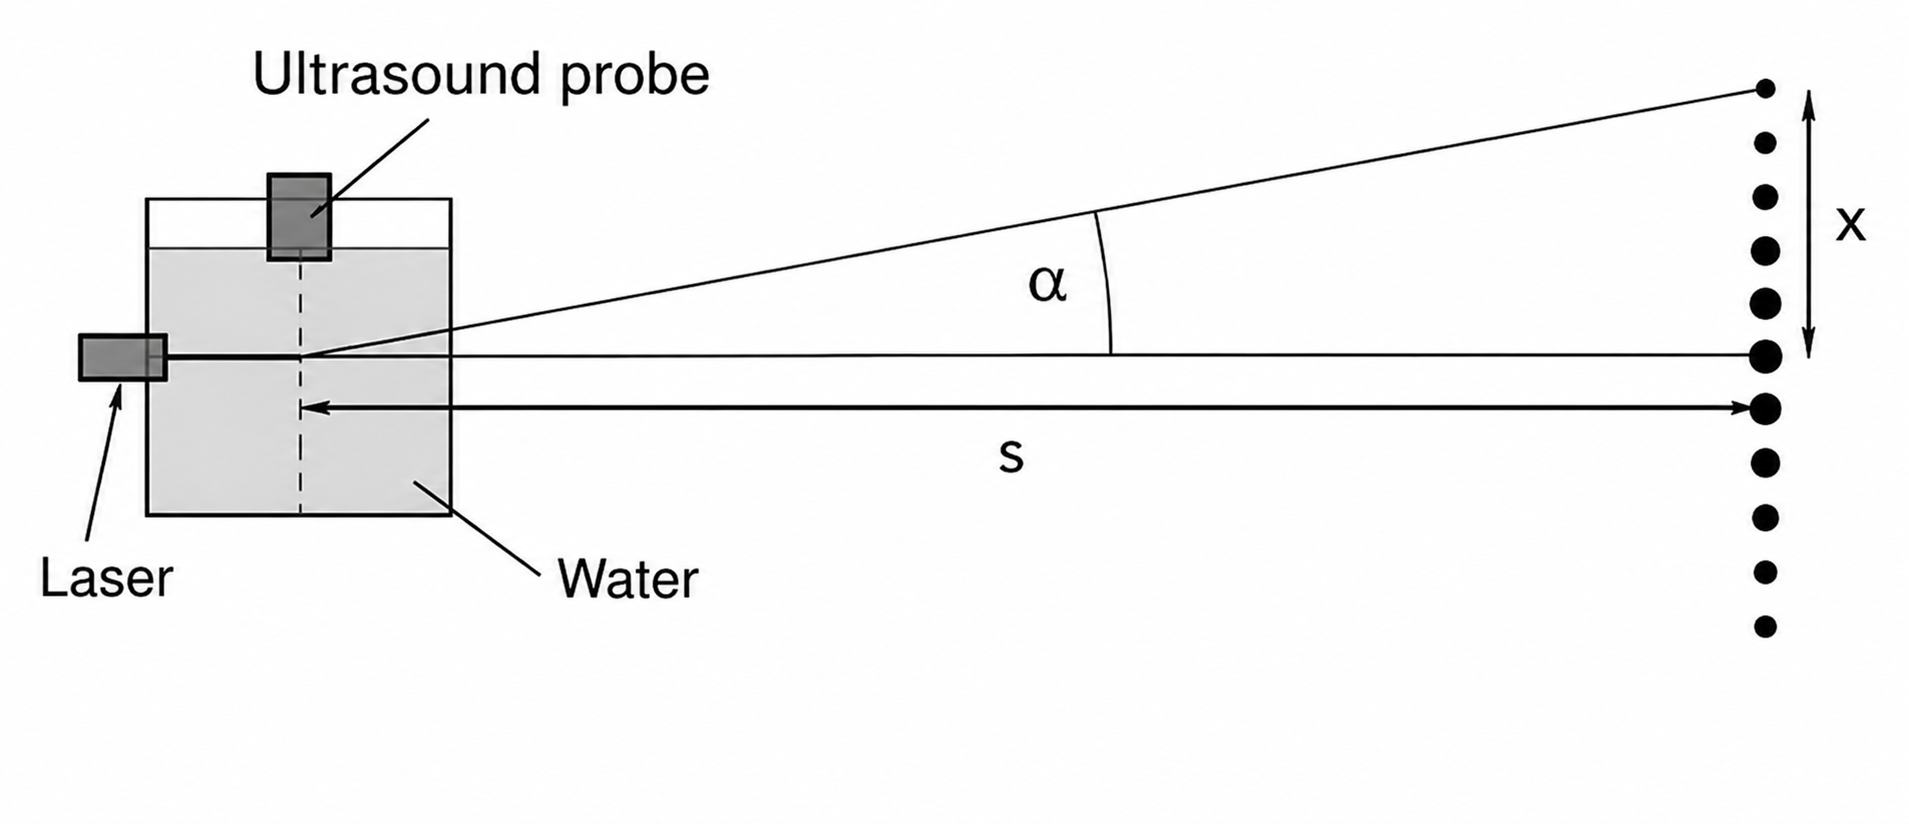
\includegraphics[width=0.5\textwidth]{../Images/setup_2.8.png}
            \caption{Setup used to measure the wavelength of ultrasound utilizing the Dabye-Sears effect}
            \label{fig:setup2.8}
        \end{figure}

        \begin{equation}
            \lambda_S = \frac{n \cdot \lambda_{laser}}{sin(\alpha)} \overset{(1)}{\approx} \frac{n \cdot \lambda_{laser} \cdot s}{x}
        \label{eq:Dabye-Sears}
        \end{equation}
        \noindent
        In eq. \ref{eq:Dabye-Sears} n is the number of the maxima, $\lambda_{laser}$ is the wavelenght of the laser and $\alpha$ is the angle of diffraction.
        The approximation (1) in eq. \ref{eq:Dabye-Sears} follows from the large difference in distance $x \ll s$. \\
        The setup of the measurement is shown in fig. \ref{fig:setup2.8}. \\
        The measured maxima distance and the calculated sound velocities for every laser wavelenght can be found in \ref{subsec:AppendixB}, \ref{tab:DataDabyeSears}.
        Using the data from tab. \ref{tab:DataDabyeSears}, the mean speed of sound could be determined as $v_{S,water} = (1438 \pm 65) m/s$. Comparing this with the
        literature value of $v_{S,lit} = 1440 m/s$ at a temperature of $T = 20 ^\circ C$, one can see that the measurement was close to the literature which
        validates the measurement method.

